%!TEX root = DT_V2_tom-mohr_martin-ohmeyer.tex
\chapter{Aufgabe 4}
\section{Aufgabe 4.1}
\paragraph{Aufgabenstellung}
Schließen Sie das Oszilloskop an den TXD Ausgang des Arduinos an. Analysieren Sie das Signal.

\paragraph{Vorbereitung}
Um den Arduino verwenden zu können, benötigt er eine Betriebsspannung von 5V, welche das Netzteil bereitstellt. Der Arduino wird mit den Pins VIN und GND mit dem Netzteil verbunden.

\paragraph{Durchführung}
Mit einem Trigger wird die Erfassung des Signals am Oszilloskop angehalten, damit es abgelesen werden kann.\\\\
\begin{tabular}{ll}
	Verwendetes Protokoll: & UART       \\
	Baudrate:              & \SI{8333}{Bd} \\
	Anzahl Stopbits:       & 1          \\
	Fehler:                & Keine Paritätsbits       \\
	Daten:                 & Das
\end{tabular}

\paragraph{Schlussfolgerung: Verwendetes Protokoll}
Bei dem verwendeten Protokoll gibt es (der Aufgabenstellung nach) zwei Möglichkeiten: DMX und RS232. Während DMX differentiell übertragen wird, ist ist dies bei RS232 nicht der Fall. In dieser Aufgabe ist das Signal nicht differentiell, weswegen es sich um \textbf{RS232} handeln muss.

\paragraph{Schlussfolgerung: Baudrate}

\mbox{}\\
\noindent
\begin{minipage}{0.5\textwidth}
	\textbf{geg.:} $f_s$ = $120 \mu s$ = $1,2 \times 10^{-4} s$
\end{minipage}%
\begin{minipage}{0.5\textwidth}
	\textbf{ges.:} $T_s$
\end{minipage}

\vspace{0.25cm}

\noindent
\textbf{Lsg:}
\begin{align*}
	T_s &= \frac{1s}{f_s} \\
	T_s &= \frac{1s}{1,2 \times 10^{-4}s} \\
	T_s &= \SI{8333,3}{Bd} \approx \SI{8,3}{kBd}
\end{align*}

\vspace{0.25cm}

\textbf{Antwort:} Die Baudrate beträgt rund $\SI{8,3}{kBd}$.

\paragraph{Schlussfolgerung: Stopbits}
Es wird ein Stopbit verwendet. Dieses ist 1.

\paragraph{Schlussfolgerung: Fehler bei der Übertragung}
Um Fehler bei der Übertragung von Daten festzustellen, gibt es drei Möglichkeiten: Die Verwendung eines Paritätsbits, die Verwendung einer Prüfsumme oder die Anwendung eines kryptografischen Verfahrens. Diese Möglichkeiten werden, in Reihenfolge ihrer Auflistung, immer sicherer, aber auch komplexer. Im Fall des während des Experimentes übertragenen Signals, kam keine Fehlerüberprüfung zum Einsatz. Anhand des Signals selbst ist folglich nicht feststellbar, ob Fehler bei der Übertragung auftraten. Nach der Auswertung der Daten ist jedoch ersichtlich: Alle Daten wurden korrekt übertragen.

\paragraph{Schlussfolgerung: Übertragene Daten}
Bei der Auswertung des Signal ist zu beachten, dass das \textit{least significant bit} zuerst und das \textit{most significant bit} zuletzt übertragen wird. Das Signal muss also "rückwärts" gelesen werden. Zur Interpretation der erhaltenen Dezimalzahlen wird die ASCII-Tabelle herangezogen. Es folgt die Analyse der ersten 30 bits des übertragenen Signals. Startbits sind grün, Stopbits rot markiert.

$$
	\textcolor{ForestGreen}{0}\underbrace{00100010}_{68 \ \equiv \ D}\textcolor{red}{1}
	\textcolor{ForestGreen}{0}\underbrace{10000110}_{97 \ \equiv \ a}\textcolor{red}{1}
	\textcolor{ForestGreen}{0}\underbrace{11001110}_{115 \ \equiv \ s}\textcolor{red}{1}
$$

\begin{figure}[h!]
	\centering
	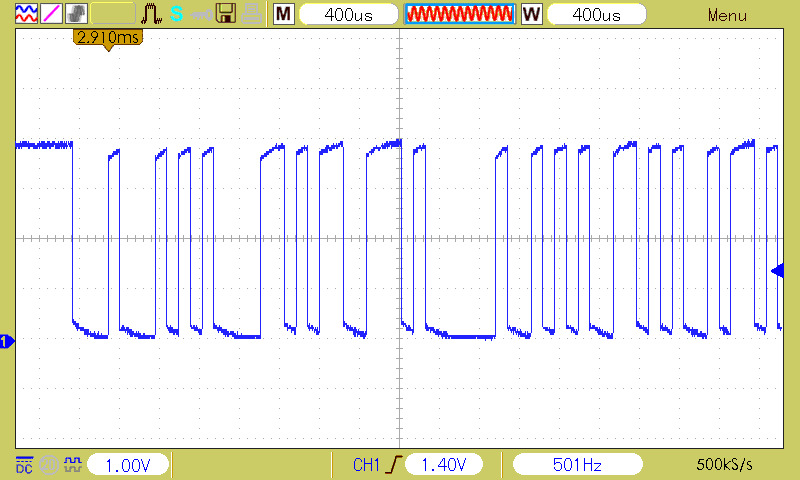
\includegraphics[width=.6\textwidth]{task4-1.jpg}
	\caption{Bildschirmfoto}
	\label{task4-1}
\end{figure}

\section{Aufgabe 4.2}
\paragraph{Aufgabenstellung}
Schließen Sie das Oszilloskop an die D+ und D- Pins des DMX-Boards an. Nutzen Sie die Mathematikfunktion um das Differenzsignal darzustellen.

\paragraph{Vorteile der differentiellen Signalübertragung}
Die differentielle Signalübertragung wird in allen modernen Protokollen verwendet. Fast alle Bussysteme, die außerhalb eines Gerätes liegen, greifen auf sie zurück. Ihre Stärke liegt in einer hohen Fehlerresistenz auch bei niedrigen Spannungen, was schnelle Übertragungsraten ermöglicht. Die Übertragung eines differenziellen Signals erfolgt dazu über zwei Kabel. Während das eine Kabel positive Spannungsausschläge verwendet, überträgt das andere Kabel negative des gleichen Betrages. Das ursprüngliche Signal wird dann durch Subtraktion der beiden einzelnen Spannungen errechnet. Der große Vorteil: Verdrillt man die beiden Kabel, so wirkt eine Störung von außen auf beide gleichermaßen. Zwar ändern sich die Spannungsausschläge, welche durch die jeweiligen Kabel übertragen werden, ihre Differenz bleibt jedoch unberührt und die übermittelten Daten unbeschädigt.

\paragraph{Durchführung}
Die Baudrate beträgt \SI{31205}{Bd}.
\\\\
\begin{tabular}{|l|l|l|l|}
	\hline
	Kanal & Binär    & Dezimal & Parameter \\ \hline\hline
	1     & 00000000 & 255     &           \\ \hline
	2     & 00000000 & 255     &           \\ \hline
	3     & 00000000 & 255     &           \\ \hline
	4     & 00000000 & 255     &           \\ \hline
	5     & 00000000 & 255     &           \\ \hline
	6     & 00000000 & 255     &           \\ \hline
	7     & 00000000 & 255     &           \\ \hline
	8     & 00000000 & 255     &           \\ \hline
\end{tabular}

\paragraph{Schlussfolgerung}


\section{Aufgabe 4.3}
\paragraph{Aufgabenstellung}
Benutzen Sie den Logicanalyser um das Zitat zu dekodieren welches der RS232-Arduino sendet.

\paragraph{Vorbereitung}
Um das Signal mittels des Logicanalyser auslesen zu können, muss dieser über einen beliebigen Kanal und GND mit dem Arduino verbunden werden. In der Anwendung PulseView wird für die Darstellung der Decoder DMX512 ausgewählt und mit dem angeschlossenen Kanal verknüpft.

\paragraph{Durchführung}


\paragraph{Schlussfolgerung}


\begin{figure}
	\centering
	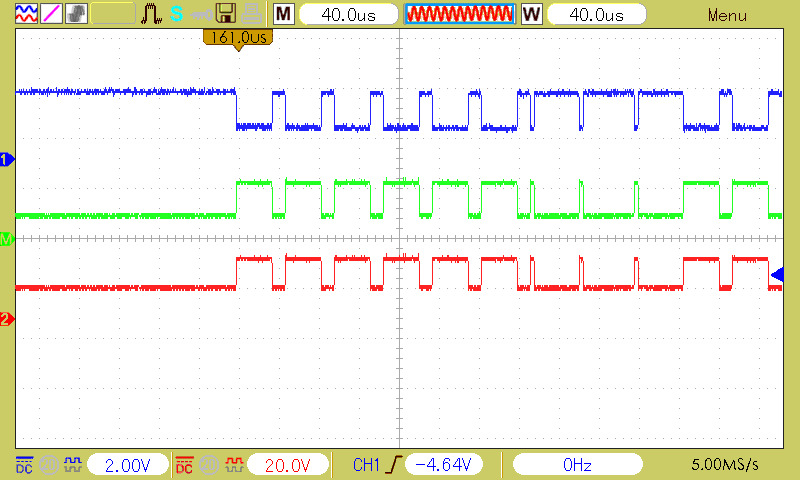
\includegraphics[width=.6\textwidth]{task4-2.jpg}
	\caption{Bildschirmfoto}
	\label{task4-2}
\end{figure}

%!TEX root = DT_V2_tom-mohr_martin-ohmeyer.tex
\section{Aufgabe 4.4}
\paragraph{Aufgabenstellung}
Wählen Sie ein Musikstück aus und programmieren Sie für die ersten 30s die Beleuchtungssequenz.

\paragraph{Vorüberlegung}
Um die DMX-Geräte ansteuern zu können, wird eine Klasse bereitgestellt, welche man mit einer einfachen Funktion, der man Adresse und gewünschten DMX-Werte gibt, bedienen kann. Da die Geräte nur an einem Ort erreichbar sind, sollte das Programm während der Entwicklung auch mit lokalen LEDs an den Pins des Arduinos ausführbar sein und einen schnellen Wechsel zwischen Test- \& Produktionsmodus ermöglichen, ohne den Code in großem Umfang abändern zu müssen. Um dies zu realisieren, werden Klassen mit Polymorphismus benötigt. Da die Geräte ihre Befehle selbstständig abarbeiten sollen, kann hier nicht mit der Delay-Funktion des Arduinos gearbeitet werden. Ein anderer Ansatz ist, fortlaufend die verstrichene Zeit ermitteln und die Objekte selbst entscheiden lassen, wann sie ihre Befehle anführen.

\paragraph{Durchführung}
In der Hauptdatei werden die Geräte als Objekte initialisiert, das DMX-Interface vorbereitet und in einer Endlosschleife die Objekte aufgerufen um ihre Befehle abzuarbeiten.
\inputminted[linenos=true, breaklines, fontsize=\fontsize{10pt}{10pt}]{cpp}{../src/main.cpp}

Damit die Geräte später einheitlich angesteuert werden können und eine gleiche Befehlsstruktur verwenden, definiert \textit{DmxCommand} die Befehle. Jeder Befehl enthält einen Zeitstempel, den Kanal und welchen Wert dieser annehmen soll.
\inputminted[linenos=true, breaklines, fontsize=\fontsize{10pt}{10pt}]{cpp}{../src/DmxCommand.h}

Um dem Polymorphismus gerecht zu werden, wird eine Basisklasse benötigt. Von \textit{DmxDevice} erben die Klassen für Scheinwerfer und Movingheads mit einer Grundstruktur von Funktionen und Variablen.
\inputminted[linenos=true, breaklines, fontsize=\fontsize{10pt}{10pt}]{cpp}{../src/DmxDevice.h}

Von dieser Basisklasse kann nun die Klasse RgbwSpotlight8Ch für die Spotlichter erben, ihre Befehle definieren und Funktionen erweitern.
\inputminted[linenos=true, breaklines, fontsize=\fontsize{10pt}{10pt}]{cpp}{../src/RgbwSpotlight8Ch.h}

Damit im Testmodus statt den Scheinwerfern LEDs verwendet werden können, erbt eine weitere Klasse \textit{RgbwSpotlight8ChDemo} von \textit{RgbwSpotlight8Ch}, um das DMX-Interface lokal emulieren zu können.
\inputminted[linenos=true, breaklines, fontsize=\fontsize{10pt}{10pt}]{cpp}{../src/RgbwSpotlight8ChDemo.h}

\paragraph{Schlussfolgerung}
Zur Kompilierzeit wird festgelegt, ob sich das Programm im Test- oder Produktionsmodus befindet. Objekte aus Klassen können in beiden Modi gleich angesteuert werden, was das testen von Befehlen stark vereinfacht. Das Programm lässt die Geräte in einer Endlosschleife selbstständig ihre Befehle abarbeiten, ohne dass diese sich durch Verzögerungen blockieren. Der Versuch ist erfolgreich.




\section{Aufgabe 4.5}
\paragraph{Aufgabenstellung}
Bitte räumen Sie auf und setzen Sie ggf. veränderte Arduinos zurück.

\paragraph{Durchführung}
Mithilfe des Befehls wird der Arduino zurückgesetzt:

\inputminted[breaklines, fontsize=\fontsize{10pt}{10pt}]{bash}{../docs/reset-dmx.txt}

\paragraph{Schlussfolgerung}
Der Arduino befindet sich in seinem Ausgangszustand und wurden Ordnungsgemäß zurück geräumt.